% $Id$
% Author: Daniel Bosk <daniel.bosk@miun.se>
\documentclass[a4paper,nocourse]{miunasgn}
\usepackage[utf8]{inputenc}
\usepackage[swedish,english]{babel}
\usepackage{url,hyperref}
\usepackage{prettyref,varioref}
\usepackage{natbib}
\usepackage[nofancy,today]{svninfo}
\usepackage{amsmath,amssymb,amsthm}
\usepackage[natbib,varioref,prettyref]{miunmisc}

\svnInfo $Id$

%\printanswers

\courseid{DT141G}
\course{Operating Systems}
\assignmenttype{Theory assignment}
\title{Processes}
\author{Daniel Bosk\footnote{%
	This work is licensed under the Creative Commons Attribution-ShareAlike 3.0 
	Unported license.
	To view a copy of this license, visit 
	\url{http://creativecommons.org/licenses/by-sa/3.0/}.
	Some of the questions are derived from the work of 
	\citeauthor*{Silberschatz2009osc}.
}}
\date{\svnId}

\begin{document}
\maketitle
\thispagestyle{foot}
\tableofcontents


\section{Aim}
\label{sec:Aim}
The aim of the assignment is, first, to aid your understanding of the treated 
content by providing questions and problems which inspire reflection.
Second, it is to examinate the following:
\begin{itemize}
	% $Id$
% Author:	Daniel Bosk <daniel.bosk@miun.se>
\item You can account for the fundamental function of the main logical 
components of an operating system, e.g.\ memory and process management, and 
explain their relations.
\item You understand the operating system interface against hardware, software, 
and users.
\item You are be able to explain the most common problems of resource 
allocation and synchronization, and be familiar with common solutions to these 
problems.
\item You can identify and understand the importance of some key parameters for 
performance in an operating system.

\end{itemize}


\section{Prerequisites}
\label{sec:Prerequisites}
% $Id$
This lecture gives an overview of the technicalities of the file system.
This is covered by Chapter 10 ``File System'' in \cite{Silberschatz2009osc}, or 
Chapter 11 ``File-System Interface'' in 
\cite{Silberschatz2013osc,Silberschatz2013intl}.



\section{Tasks}
\label{sec:Tasks}
\begin{questions}
	\question\label{q:processthread}
	Define the terms
	\begin{parts}
		\part process, and
		\part thread.
	\end{parts}
	(What is the difference between them?)
	\begin{solution}
		A \emph{process} is a running instance of a program \citep[p.  
		102]{Silberschatz2009osc}.
		From the view of the operating system it consists of everything needed to 
		handle the execution of a program; memory, a pointer to where in the code 
		it is currently executing, etc.

		According to \citet[pp. 153--154]{Silberschatz2009osc} \emph{thread} is 
		quite similar to a process.
		By thread we mean ``thread of execution'', thus the process above has one 
		thread of execution -- it is a single-threaded process.
		Adding more threads to a process means that we add more threads of 
		execution, we need more pointers to know where each thread is currently 
		executing.
		But these threads still share the memory and everything else within the 
		process.

		Starting a new process, however, means that we allocate new memory etc.  
		making the two processes completely independent from eachother.
	\end{solution}

	%%% SCHEDULING %%%

	\question\label{q:scheduling}
	A CPU scheduling algorithm determines an order for the execution of its 
	processes.
	Given \(n\) processes to be scheduled on a single-core processor, how many 
	possible different schedules are there?
	\begin{solution}
		There are \(n! = n\cdot n-1\cdot \ldots\cdot 2\cdot 1\) as we can first 
		choose any of the processes, then any of the remaining, and so on.
	\end{solution}

	\question\label{q:scheduler}
	Define the different levels of process scheduling,
	\begin{parts}
		\part short-term,
		\part medium-term, and
		\part long-term.
	\end{parts}
	(What is the difference between them?)
	\begin{solution}
		\citet[p. 108]{Silberschatz2009osc} defines the \emph{long-term} scheduler 
		as the scheduler which selects the jobs which will be allowed to start 
		their execution.
		Thus, the long-term scheduler is the scheduler controlling the degree of 
		multiprogramming, i.e.\ the number of processes which are kept in memory.

		The \emph{short-term} scheduler, also known as the \emph{CPU scheduler}, 
		selects among the jobs waiting in memory ready to execute and allocates the 
		CPU to one of them \citep[p. 108]{Silberschatz2009osc}.

		The \emph{medium-term} scheduler does the opposite of the long-term 
		scheduler.
		It removes processes from memory to decrease the degree of multiprogramming 
		when needed \citep[p. 109]{Silberschatz2009osc}, this is called 
		\emph{swapping} \citep[p. 109]{Silberschatz2009osc}.
	\end{solution}

	\question\label{q:schedulingalgs}
	Describe how the following scheduling algorithms work and their advantages 
	and disadvantages:
	\begin{parts}
		\part first-come first-served (FCFS),
		\part shortest-job-first (SJF),
		\part priority,
		\part round-robin (RR),
		\part multi-level queue (MLQ), and
		\part multi-level feedback queue (MLFQ),
	\end{parts}
	\begin{solution}
		FCFS works in a very straight-forward fashion, all processes are scheduled 
		as they are arrived using a simple first-in first-out queue \citep[p.  
		188]{Silberschatz2009osc}.
		The main disadvantage of this algorithm is that the waiting-time can be 
		long \citep[see][bottom p. 188]{Silberschatz2009osc}.

		The purpose of SJF is to counter the disadvantage of long waiting in FCFS.
		In this algorithm the shortest job is scheduled to run first thus 
		minimizing the waiting time for all processes \citep[p.  
		190]{Silberschatz2009osc}.
		The obvious problem with this algorithm is that it is very hard to estimate 
		the running-time of each process, hence making it impossible to know which 
		one to schedule before another.

		\citet[p. 192]{Silberschatz2009osc} defines the priority scheduling 
		algorithm as follows.
		It has all processes associated with a given priority, say either high or 
		low.
		The high-priority processes are then scheduled before the low-priority 
		ones.
		When choosing between two processes of the same priority the FCFS algorithm 
		may be used.

		An obvious disadvantage with priority scheduling is the starvation of 
		low-priority processes.
		However, this can be countered by having low-priority processes age into 
		high-priority processes, this way they will eventually be allowed to 
		execute \citep[p. 193]{Silberschatz2009osc}.

		Round-robin scheduling is an extension of FCFS which adds preemption 
		\citep[p. 194]{Silberschatz2009osc}.
		This way the CPU-scheduler can switch between running processes.
		A process may run for the duration of a time quantum or slice.
		If the process has not finished by the end of the time slice is it 
		preempted and put back to the tail of the queue.

		A drawback is that waiting-time again increases \citep[p.  
		192]{Silberschatz2009osc}, depending on the time quantum chosen.
		Another drawback is that overhead is added to handle preemption.

		According to \citet[pp. 196--197]{Silberschatz2009osc} a \emph{multilevel 
		queue} scheduling algorithm partitions the ready-queue into separate queues 
		with different priorities.
		Each of these queues has its own scheduling algorithm and a scheduling 
		algorithm is also needed to schedule the different queues.
		This is simply a generalization of the priority scheduling algorithm, this 
		version supports different scheduling algorithms within the queues and it 
		also allows preemption.
		The disadvantage is that processes are fixed to a certain queue, a process 
		cannot move from one queue with lower priority to another with higher 
		priority (nor the other way around).

		The \emph{multilevel feedback queue} scheduling solves this problem.
		In this kind of scheduling we can actually solve the problem with aging as 
		we did with the priority queue \citep[cf.][p. 198]{Silberschatz2009osc}.
	\end{solution}

	\question\label{q:roundrobin}
	Given this variant of the round-robin scheduling algorithm, where the entries 
	in the ready queue are pointers to the PCBs, what would be the effect of 
	putting two pointers to the same PCB in the ready queue?
	\begin{solution}
		Given how round-robin works \citep[pp. 194-195]{Silberschatz2009osc}, the 
		process in question would get a higher priority than other processes as 
		this one will be scheduled twice as often as other processes -- as it has 
		two entries in the ready queue.
	\end{solution}

	\question\label{q:favouringalg}
	Consider a short-term scheduling algorithm which favours processes that have 
	used the least processor time in the recent past.
	Why will this algorithm favour I/O-bound processes and yet not starve 
	CPU-bound processes?
	\begin{solution}
		Because the processes are I/O-bound they will have to break waiting for 
		I/O-devices, usually after a short burst, then they will relinquish the 
		processor for use by other processes.
		CPU-bound processes will thus not starve as I/O-bound processes will do I/O 
		quite often.
	\end{solution}

	\question\label{q:threads}
	Describe the different ways of implementing threads, e.g. user threads and 
	kernel threads.
	(What is the difference between them, what advantages and disadvantages are 
	there with the different methods?)
	\begin{solution}
		The advantage of user threads is that an application can use them without 
		support in the operating system.
		The disadvantage is thus that the process scheduler is unaware of the fact 
		that more than one thread is executing within a process and hence all 
		threads will share the process time quantum.
		Another disadvantage is that of system calls (e.g. I/O).
		From the view of the operating system a single-threaded process made 
		a system call and is then suspended until the call completes.
		However, if the process used a user space threading library all threads 
		will be blocked.

		If the operating system supports threads by scheduling each thread 
		independently of its process, e.g. by using kernel threads, then two 
		threads could be scheduled to run on different cores in a multi-core 
		system.
		They could also be scheduled on separate processors, however, this would 
		mean that the caches of two processors must be synchronized.
	\end{solution}

	%%% SYNCHRONIZATION %%%
	
	\question\label{q:criticalsection}
	State and explain the requirements of the critical-section problem.
	\begin{solution}
		To ensure a race condition does not occur we have to solve the 
		critical-section problem.
		\citet[p. 228]{Silberschatz2009osc} states the following requirements, 
		which all must be satisfied to avoid a race condition:
		\begin{description}
			\item[Mutual exclusion] No two processes must simultaneously be in their 
				critical sections.
			\item[Progress] Only the processes which are not in their remainder 
				sections may participate in the decision of which process may enter 
				their critical section.
				This way even a selfish algorithm will allow all processes to 
				eventually enter their critical section.
			\item[Bounded waiting] There must exist an upper bound on how long 
				a process may wait before entering its critical-section after a request 
				to do so.
				This way we avoid starvation.
		\end{description}
	\end{solution}

	\question\label{q:multicore}
	Describe the problems which need to be handled for multi-processor and 
	multi-core processor systems.
	\begin{solution}
		E.g. having synchronized caches, a process is swapped out from one 
		processor and then swapped in to another.
		Or having a multi-core processor with a shared cache, where each executing 
		core can modify the common cache.
	\end{solution}

	%%% DEADLOCKS %%%

	\question\label{q:deadlock}
	State and explain the requirements for a deadlock to occur.
	\begin{solution}
		\citet[pp. 285--287]{Silberschatz2009osc} states that a deadlock can occur 
		only if these four conditions holds simultaneously:
		\begin{description}
			\item[Mutual exclusion] There must be at least one resource which is 
				locked for use by a single process.
			\item[Hold and wait] All processes in the deadlock must be holding at 
				least one resource and be waiting to acquire another held by another 
				process.
			\item[No preemption] A process holding a resource does not release it 
				until the task is completed, i.e.\ after all other resources are also 
				acquired.
			\item[Circular wait] All processes in the deadlock must be waiting for 
				each other.
				If we have the set of processes \(\{P_0, P_1, \ldots, P_N\}\) then
				process \(P_0\) must be waiting for a resource held by process \(P_1\), 
				process \(P_1\) must be waiting for \(P_2\), and so on until process 
				\(P_N\) which is waiting for \(P_0\).
		\end{description}
		If only one of these conditions does not hold a deadlock cannot occur, i.e.\  
		to prevent deadlocks we must ensure that one of these conditions cannot 
		hold.
	\end{solution}

	\question\label{q:deadlockfree}
	Consider a system of four resources, all of the same type, that are shared by 
	three processes, each of which needs at most two of the resources.
	Show that the system cannot enter a deadlock.
	\begin{solution}
		This is easily proved by contradiction.
		Assume the system is deadlocked.
		This implies that each process holds one resource and is waiting for one 
		more.
		As there are four resources but only three acquired by processes, one of 
		the four resoures must be free for one of the three processes to acquire.
		(This contradicts the requirement for circular waiting.)
		Hence, when that process finishes resources will be freed for the others.
		A deadlocked state can thus never occur.
	\end{solution}

	%%% GENERAL %%%

	\question\label{q:sleepingrouter}
	The problem presented here is an adaption of the sleeping barber problem and 
	the producer-consumer problem, we can call it the sleeping-router 
	problem\footnote{%
		This model applies on many things, e.g. a physical router and on a virtual 
		machine with one physical device and many virtual devices.
	}.
	The problem is simplified in that traffic only flows in one direction.
	There are four network interfaces to which data arrive from different 
	networks, there is also one interface through which all data eventually 
	leaves.
	See \prettyref{fig:router}.
	Each interface and the box in the middle may have a small buffer keeping only 
	a few packets.
	The problem is to guarantee the system is synchronized, without starvation, 
	and that no deadlocks can occur.
	Describe what buffers, locks, etc. which are needed to make this work.
	\begin{figure}
		\centering
		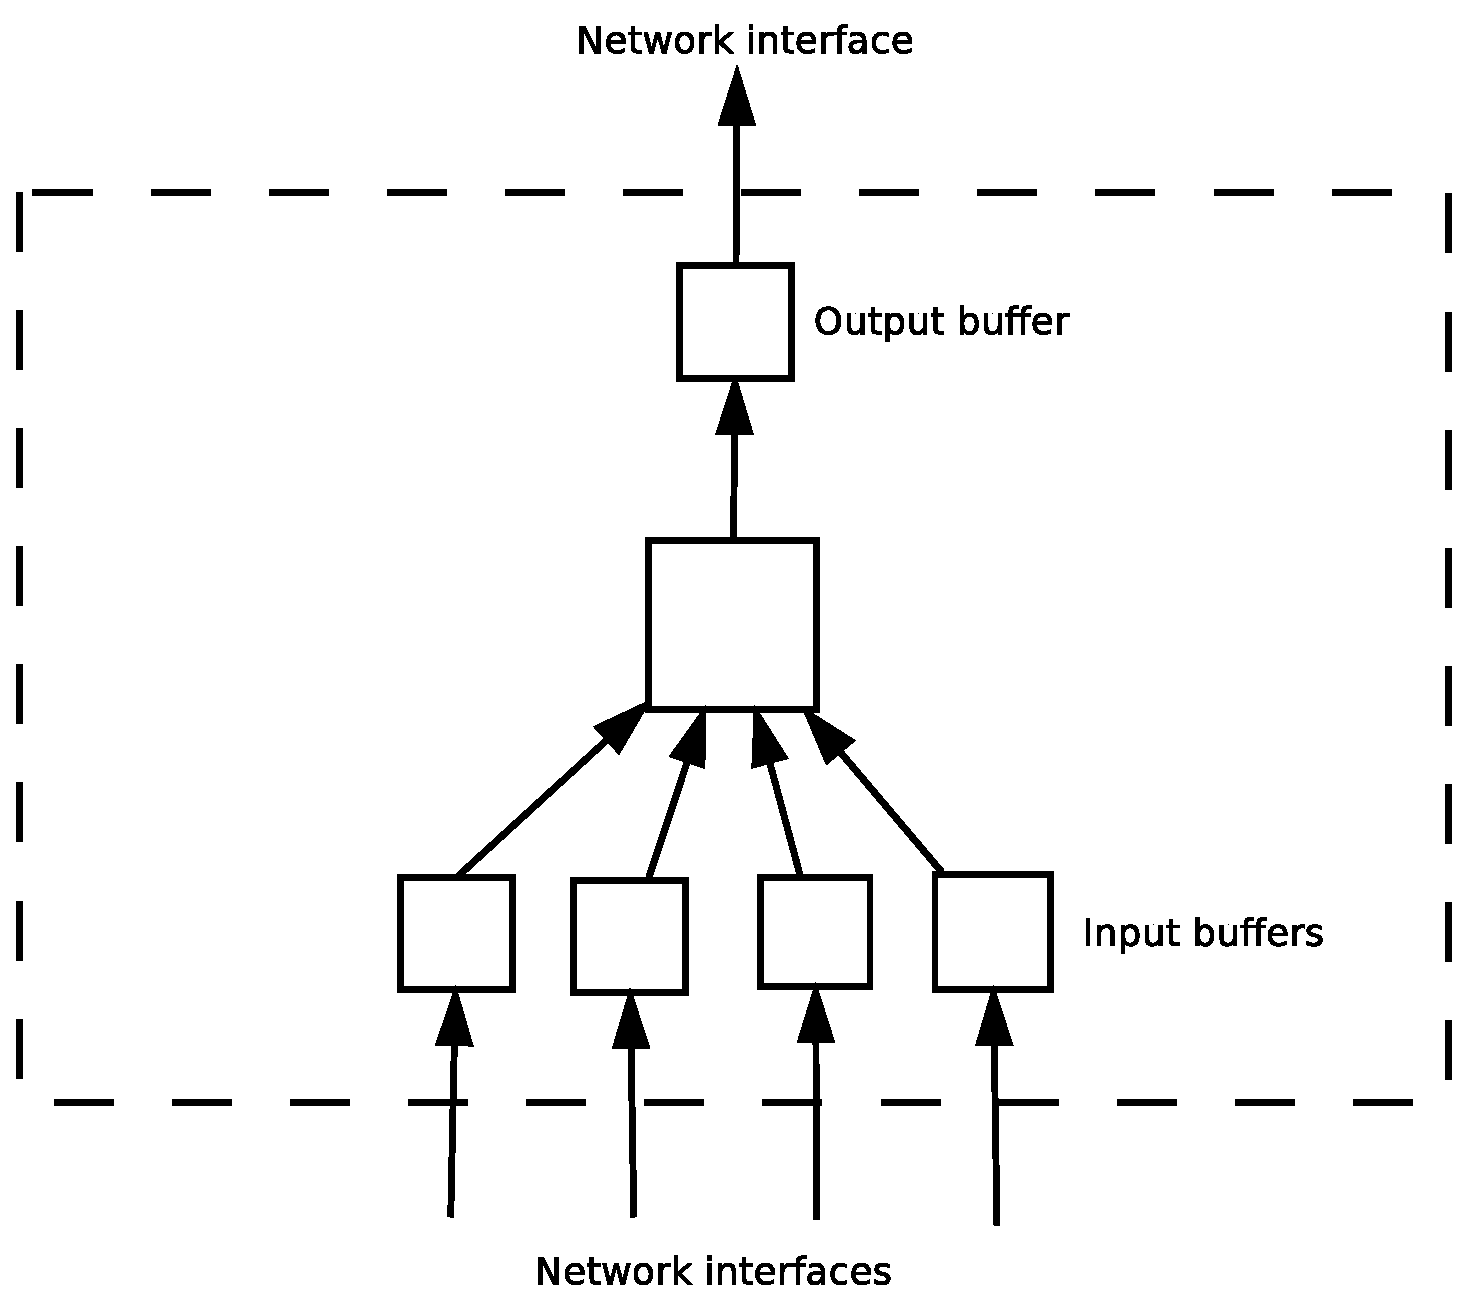
\includegraphics[width=0.7\linewidth]{router.eps}
		\caption{A general depiction of a router or switch with five network 
		interfaces and the data flowing from bottom to top.}
		\label{fig:router}
	\end{figure}
	\begin{solution}
		This question is open, there is no given answer.
		The point here is to convincingly prove (e.g. using the requirements for 
		deadlocks and the critical-section problem) that neither a deadlock nor 
		a race condition can occur in the system.

		The problem to be solved is essentially one instance of the bounded-buffer 
		problem \citep[see][sec. 6.6.1]{Silberschatz2009osc} for each of the 
		buffers in the system.

		One way of solving it is to protect each buffer with a mutex lock and two 
		counting semaphores.
		One semaphore indicating how many empty and one indicating how many full 
		places are in the buffer.

		The producer of the packets first wait for the empty-semaphore.
		Once acquired it waits for the mutex lock.
		The producer can now enter its critical section, i.e.\ writing a packet to 
		the buffer.
		Once done it can release the mutex lock and then signal the full-semaphore.
		It has completed its update of the buffer.

		When the consumer of a buffer wishes to get a packet from the buffer it 
		first waits for the full-semaphore.
		It then acquires the mutex lock and reads a packet from the buffer.
		The mutex lock is released and it signals the empty-semaphore.

		We first show the critical-section problem is solved.
		This is done by showing that the requirements from \citet[p.  
		228]{Silberschatz2009osc} are satisfied.

		\begin{proof}
			The mutex lock ensures that the mutual exclusion requirement holds.
			Assume that one of the two processes, either the producer or consumer, is 
			starved by the other.
			If the consumer is starved, then only the producer gets access to the 
			buffer.
			However, when the buffer becomes full the producer must wait for the 
			empty-semaphore.
			While waiting for the semaphore the mutex is not locked and the consumer 
			can access the buffer.
			Hence the requirement for bounded waiting is satisfied.
			As the consumer then signals the empty-semaphore the producer is allowed 
			back into the buffer.
			Thus also providing the requirement for progress.
			
			The same argument applies the other way around.
		\end{proof}

		We now show there can be no deadlock.
		This is done by showing that at least one of the conditions for a deadlock 
		given by \citet[pp. 285--287]{Silberschatz2009osc} is never satisfied.

		\begin{proof}
			Assume that both processes are waiting to enter their critical section 
			and both holds one of the resources required, i.e.\ all conditions for 
			a deadlock are satisfied.
			This must mean that both has successfully waited for their semaphores and 
			are thus waiting for the mutex lock.
			As neither has acquired the lock it cannot be locked and one of them will 
			acquire it.
			The process which acquires it will then execute its critical section and 
			then its remainder section, thus there is no circular waiting and hence 
			there can be no deadlock.
		\end{proof}
	\end{solution}

\end{questions}


%%% EXAMINATION %%%
\input{examination.tex}


\bibliography{literature}
\end{document}
